\chapter{Resultados}

\noindent Este capítulo apresenta os resultados qualitativos e quantitativos obtidos durante o desenvolvimento e implantação do ``\acrshort{uft} Serviços'' e, para um melhor entendimento destes, este tópico foi dividido em quatro seções principais, sendo elas: Acordo de Nível de Serviço (\acrshort{gps}), O Software, Resultados dos Testes Realizados e Ferramentas de Monitoramento.

Na seção Acordo de Nível de Serviço (SLA) é explicada a utilização deste documento e as informações contidas nele. A seção O \textit{Software}, por sua vez, apresenta as principais telas e funcionalidades do sistema ``\acrshort{uft} Serviços'', tanto do sistema móvel Android como também do sistema \textit{web} administrativo. Em Resultado dos Testes Realizados são apresentados os resultados obtidos pela aplicação dos Testes de Usabilidade SUS, Teste de Desempenho e Teste de Segurança. Por fim, em Ferramentas de Monitoramento são expostos os resultados obtidos durante a verificação do comportamento do \textit{software} em produção e dos usuários durante a utilização do aplicativo móvel.

\section{Acordo de Nível de Serviço (SLA)}

\noindent Para a implantação do sistema UFT Serviços foi criado um acordo de nível de serviço (SLA) , para a realização do gerenciamento do nível de serviço descrito na etapa de Desenho de Serviço do ITIL v3. A \acrshort{sla} construída contém informações gerais de uma acordo de nível de serviço, tais como o Acordo Geral, as Metas e Objetivos, os Responsáveis, o Ambiente do Serviço, a Revisão Periódica, Contrato , gerenciamento e custos de Serviços. Como pode ser observado no Apêndice III, é apresentado o \acrshort{sla} criado para firmar o acordo de nível de serviço entre os envolvidos no projeto com o Campus Universitário de Palmas da Universidade Federal do Tocantins quanto a prestação de serviço do sistema desenvolvido neste trabalho.

\section{\textit{O Software}}

\noindent Para apresentar o sistema foi realizada a captura de algumas de suas telas, sendo que as apresentadas neste trabalho correspondem às mais utilizadas pelos usuários do aplicativo móvel Android e pelo sistema \textit{web} administrativo.

Para um melhor entendimento e compressão das informações a serem apresentadas nesta seção, ela foi subdividida em : Sistema \textit{Mobile} e Sistema \textit{web}. No primeiro título, apresenta-se a versão do sistema ``\acrshort{uft} Serviços'' para dispositivos Android, apresentando as telas do aplicativo em funcionamento em aparelhos como \textit{smartphone} e \textit{tablet}. Em Sistema \textit{web} tem-se a apresentação do sistema administrativo para o gerenciamento dos chamados realizados a partir do aplicativo móvel, contendo as  telas de autenticação do usuário administrador, a tela inicial do sistema e a caixa de diálogo utilizada para o encaminhamento dos chamados.

O resultado deste trabalho foi a concepção do sistema de informação ``\acrshort{uft} Serviços'', apresentado na Figura \ref{diagram-uml-casodeuso} através de um caso de uso geral com as ações que podem ser realizadas através da interação dos usuários com o mesmo.

\subsection*{Sistema \textit{Mobile}}

\noindent Na Figura \ref{start-uftservicos} podem ser observadas as telas de \textit{login} do usuário e a tela principal do aplicativo, além dos chamados realizados pelo usuário listados em três principais categorias, sendo elas: Chamados em Aberto, Em Atendimento e Concluído.

\begin{figure}[H]
\centering
    \begin{tabular}{cc}
     \includegraphics[width=0.3\textwidth]{figuras/applogin_uftservicos.png}  &  \includegraphics[width=0.3\textwidth]{figuras/appstart-chamadoaberto-uftservicos.png} 
    \end{tabular}
    \caption{Tela inicial e de login aplicativo ``\acrshort{uft} Serviços'' \textit{Smartphone}.}
    \label{start-uftservicos}
\end{figure}

Na tela de formulário o usuário tem a possibilidade de realizar o envio da foto do chamado a partir da câmera do aparelho ou pela galeria de fotos, apresentando o local em que ocorreu com o \acrshort{gps} do aparelho. Na tela de detalhes do chamado o usuário pode visualizar a foto do problema, o local, uma breve descrição, as providências a serem tomadas, um campo de observações do chamado e o \textit{e-mail} de contato do atendente da solicitação, conforme a Figura \ref{form-uftservicos}.

\begin{figure}[H]
\centering
    \begin{tabular}{cc}
     \includegraphics[width=0.3\textwidth]{figuras/appform-chamado-uftservicos.png}  &  \includegraphics[width=0.3\textwidth]{figuras/appstart-chamadodetalhes-uftservicos.png} 
    \end{tabular}
    \caption{Tela de formulário de abertura do chamado e de visualização dos detalhes do chamado enviado pelo \textit{Smartphone}.}
    \label{form-uftservicos}
\end{figure}

As Figuras \ref{tabapp-login} e \ref{tabapp-start} mostram a tela de \textit{login} e os chamados em funcionamento em um \textit{Tablet}. Como pode ser observado, o mesmo aplicativo desenvolvido para \textit{smartphone} se adequada de forma satisfatória em um dispositivo de maior resolução de tela, como um \textit{Tablet}. Este fato, é de grande importância, devido a praticidade que o dispositivo proporciona para uma visualização mais ampla das informações.

\begin{figure}[H]
  \centering
  \includegraphics[width=0.7\textwidth]{figuras/tabapp-login-uftservicos.png} 
  \caption{Tela de Login aplicativo ``\acrshort{uft} Serviços'' Tablet.}
  \label{tabapp-login} 
\end{figure}

\begin{figure}[H]
  \centering
  \includegraphics[width=0.7\textwidth]{figuras/tabapp-start-uftservicos.png} 
  \caption{Tela inicial aplicativo ``\acrshort{uft} Serviços'' Tablet.}
  \label{tabapp-start} 
\end{figure}

\subsection*{Sistema web}

\noindent As Figuras \ref{web-start} e \ref{web-atendimento} mostram as telas de \textit{login} do sistema administrativo do ``\acrshort{uft} Serviços'', a tela inicial do sistema \textit{web} e a caixa de diálogo de atendimento dos chamados realizados a partir do aplicativo móvel. Além disso, na Figura \ref{web-start}, é possível observar os \textit{links} existentes para as funcionalidades como a geração de relatório, gerenciamento de pessoas administrativas, gerenciamento de categorias e gerenciamento dos blocos.

\begin{figure}[H]
  \centering
  \includegraphics[width=0.7\textwidth]{figuras/web-telainicial-uftservicos.png} 
  \caption{Tela inicial do Sistema \textit{web} administrativo ``\acrshort{uft} Serviços''.}
  \label{web-start} 
\end{figure}

\begin{figure}[H]
  \centering
  \includegraphics[width=0.7\textwidth]{figuras/web-atendimento.png} 
  \caption{Caixa de dialogo atendimento do chamado Sistema \textit{web} administrativo ``\acrshort{uft} Serviços''.}
  \label{web-atendimento} 
\end{figure}

\section{Resultado dos Testes Realizados}

\noindent Nesta seção é apresentado os resultados obtidos pela realização dos Teste de Usabilidade, Teste de Desempenho e Teste de Segurança. Onde cada um dos testes realizados foram fundamentais para a averiguação dos resultados obtidos pelo desenvolvimento do sistema ``\acrshort{uft} Serviços''. Com a realização dos testes foi a constatação de itens como a facilidade de utilização do sistema, o desempenho e a segurança das requisições realizadas no sistema.

\subsection*{Teste de Usabilidade}

\noindent A realização dos testes de usabilidade é um dos pontos fundamentais dentre os resultados obtidos pela realização deste trabalho. Foi através da realização deste teste que foi possível fazer uma análise sobre os níveis de satisfação dos usuários com o sistema. Fornecendo também outras informações como a facilidade, a eficiência e se os usuários se sentem confortáveis em estar utilizando o sistema em um primeiro contato.

O teste de usabilidade foi aplicado em um grupo com 80 voluntários, sendo 16 professores, 16 técnicos administrativos e 48 alunos, sendo a idade dos voluntários entre 18 a 59 anos de ambos os sexos. O Apêndice IV demonstra em detalhes o perfil dos usuários em que o teste foi aplicado.

Definiu-se previamente que a aplicação do teste seria através da execução de sete atividades no sistema em que os participantes deveriam desempenhar. Cada uma das atividades realizadas pelos voluntários foram feitas de forma que não houvesse nenhum contato anterior com o sistema, sendo apenas informado brevemente sobre qual era o objetivo do \textit{software} desenvolvido. As atividades definidas para execução dos voluntários do teste foram as seguintes:

\begin{itemize}
    \item \textbf{Tarefa 1}: Cadastro do usuário no sistema, ativação do usuário no \textit{e-mail} e autenticação no sistema;
    \item \textbf{Tarefa 2}: Abertura de um novo Chamado;
    \item \textbf{Tarefa 3}: Visualização do chamado na tela principal do aplicativo;
    \item \textbf{Tarefa 4}: Edição ou exclusão de um chamado;
    \item \textbf{Tarefa 5}: Acompanhamento da mudança de estágio do chamado;
    \item \textbf{Tarefa 6}: Visualização dos gráficos dos chamados realizados; e 
    \item \textbf{Tarefa 7}: Encerramento de sessão do usuário no aplicativo.
\end{itemize}

Para fins de avaliação sobre a facilidade de utilização do sistema, todas as atividades executadas pelos usuários foram cronometradas. O objetivo desta abordagem é que fosse possível ao final da realização do teste de usabilidade a verificação do tempo médio de execução de cada uma das tarefas executadas. 

Ao final da aplicação do SUS foi obtido o resultado médio igual a 87,1 pontos, o que classifica o sistema desenvolvido como excelente no quesito usabilidade. A Figura \ref{time_task} e \ref{time_pizza} apresenta o tempo médio em que os voluntários levaram para executar todas as atividades propostas pelo teste. Como pode ser observado, a maior parte do tempo de execução do teste do usuário está na realização do seu cadastro no sistema (Tarefa 01) e no processo de abertura do chamado (Tarefa 02).

\begin{figure}[H]
  \centering
  \includegraphics[width=1\textwidth]{figuras/time_task.png} 
  \caption{Gráfico do tempo médio de execução das tarefas realizadas pelos voluntários.}
  \label{time_task} 
\end{figure}

\begin{figure}[H]
  \centering
  \includegraphics[width=1\textwidth]{figuras/time_pizza.png} 
  \caption{Gráfico de Pizza do tempo médio de execução das tarefas realizadas pelos voluntários.}
  \label{time_pizza} 
\end{figure}

O tempo médio total para realização de todas as tarefas foi de 07 minutos e 45 segundos, o que pode ser considerado um bom tempo de execução visto que os voluntários desempenharam todas as principais atividades disponíveis no aplicativo móvel.

\subsection*{Teste de Desempenho}

\noindent Dentre os testes realizados no sistema ``\acrshort{uft} Serviços'', o de desempenho se mostrou um dos mais relevantes em sua aplicação. 

Para a aplicação do teste de desempenho foi feita a verificação do comportamento do sistema em suportar o acesso de 1000 usuários simultaneamente, através da ferramenta de código aberto JMeter\footnote{JMeter: http://jmeter.apache.org/} para simular as requisições de acesso ao sistema.Foram utilizadas também duas máquinas virtuais hospedadas nos servidores da Digital Ocean\footnote{Digital Ocean: http://digitalocean.com}, cujas configurações de \textit{hardware} utilizadas como base para a realização do teste é apresentada na Tabela \ref{tbl_config_desempenho}.

\begin{table}[!h]
\centering
\begin{tabular}{|l|c|c|}
\hline
\multicolumn{1}{|c|}{Item} & \multicolumn{1}{l|}{Servidor de Aplicação} & \multicolumn{1}{l|}{Servidor de Banco de Dados} \\ \hline
RAM                        & 1GB DDR3                                   & 512 MB DDR3                                     \\ \hline
Processador                & 1 CPU                                      & 1 CPU                                           \\ \hline
HD                         & 30 GB SSD                                  & 20 GB SSD                                       \\ \hline
\end{tabular}
\caption{Configuração servidores de aplicação e banco de dados ``\acrshort{uft} Serviços''.}
\label{tbl_config_desempenho}
\end{table}

Foram necessárias configurações no servidor de aplicação para obtenção de um melhor desempenho da aplicação em produção, uma das configurações realizadas diz respeito ao \textit{pool} de conexão do servidor Wildfly, com o intuito de obter um melhor tempo de resposta com relação as consultas no banco de dados.

A aplicação do teste de desempenho utilizado neste trabalho consistiu na execução de simulações das requisições HTTP realizadas na aplicação REST API. Nesse aspecto, foi feita a simulação de acesso de mil usuários simultâneos requisitando o acesso ao sistema de autenticação utilizado pelo aplicativo móvel do sistema ``\acrshort{uft} Serviços''.

A Figura \ref{login_rest} mostra o resultado obtido com o teste de desempenho em relação ao sistema de autenticação da aplicação REST API, no qual foi possível verificar que o tempo total para sua execução foi de apenas 8 segundos, que corresponde à um resultado excelente para a quantidade de acesso. Outro ponto que pode ser observado é a vasão de 5.696,924/minuto do site, o que significa a quantidade de operações por minuto que o sistema pode realizar durante este período de tempo, apresentando também um desvio padrão 50 com relação ao tempo total decorrido durante a realização do teste.

\begin{figure}[!h]
  \centering
  \small
  \includegraphics[width=1\textwidth]{figuras/login_rest.png} 
  \caption{Resultado teste de desempenho Login API REST.}
  \label{login_rest} 
\end{figure}


\subsection*{Teste de Segurança}

A segurança da informação é um dos principais itens que foram testados no sistema ``\acrshort{uft} Serviços'', em que decidiu-se pela utilização dos testes de caixa preta e caixa branca como base para execução do teste de segurança. O motivo da escolha da aplicação destes testes,  é a sua simplicidade de utilização e sua eficiência quanto a verificação da existência de vulnerabilidades no sistema que comprometam a segurança.

A aplicação do teste de Caixa Preta consiste em verificar a existência de falhas com relação ao levantamento de requisitos do sistema, sendo que para a realização do teste é verificado o funcionamento de toda a aplicação através da simulação da inserção de entradas inválidas no sistema.

Para a realização do teste de caixa preta, foi utilizado a ferramenta para automação do teste chamada Selenium\footnote{Selenium: http://www.seleniumhq.org/}. A utilização desta ferramenta é feita através da simulação de um caso de uso de uma dada atividade do usuário no sistema, onde a atividade a ser executada pela ferramenta é feita através automatização do teste a partir da criação de um \textit{script} que descreve todas as ações a serem executadas pelo Selenium.

A Figura \ref{caixa_branca} demonstra o exemplo de aplicação do teste de caixa preta realizado no sistema de autenticação do sistema \textit{web} administrativo do ``\acrshort{uft} Serviços'', em que pode ser observado o teste para validação da entrada de um usuário e senha no sistema.

\begin{figure}[H]
  \centering
  \small
  \includegraphics[width=0.7\textwidth]{figuras/selenium_test.png} 
  \caption{Teste de Caixa Branca utilizando o Selenium.}
  \label{caixa_branca} 
\end{figure}

O processo descrito consiste em simular a entrada do \textit{e-mail} do usuário e senha para que então sejam validadas as informações da entrada no sistema de autenticação do ``\acrshort{uft} Serviços'', sendo observado o comportamento do sistema quanto a entrada de informações inválidas.

Foram simuladas entradas de usuário e senha tanto de usuários que tem acesso ao sistema administrativo como do usuários que não tem a permissão de acesso, sendo testado também a inserção de informações inválidas no sistema, como por exemplo, a entrada de um \textit{e-mail} válido e uma senha incorreta e a entrada de um \textit{e-mail} inválido com uma senha válida.  Observou-se durante os testes que não há excessões neste processo.  exceção.

O teste de Caixa Branca tem como propósito testar as partes internas do \textit{software} a procura de eventuais falhas de modelagem que possam expor vulnerabilidades com relação a segurança do sistema. Para a aplicação do teste de caixa branca foi realizado uma bateria de testes unitários, sendo catalogado todos os que falharam para verificação de alguma brecha de segurança.

Para a realização do teste de caixa branca foi utilizada a aplicação de teste unitário. Este teste consiste na verificação do comportamento do método de autenticação do sistema ao inserir valores de \textit{login} e senha corretos, bem como a inserção de informações incorretas de autenticação.

O Apache Maven foi utilizado para execução do teste durante o processo de compilação da aplicação, sendo que em caso de ocorrência de falhas a aplicação não conclui a etapa de compilação do projeto.

Foi possível constatar que durante a execução do teste não houve a ocorrência de nenhuma falha que tenha exposto alguma vulnerabilidade do sistema de autenticação do ``\acrshort{uft} Serviços''. A aplicação do teste de caixa branca neste caso foi bastante útil para verificação do comportamento do sistema durante a inserção de entradas inválidas.

\section{Ferramentas de Monitoramento}

\noindent Para que um sistema tenha um bom funcionamento ele deve estar implantado em um servidor que satisfaça os requisitos mínimos para que o sistema funcione adequadamente, por este motivo, optou-se pelo uso de sistema de monitoramento com relação utilização do \textit{hardware} e de rede pelo sistema ``\acrshort{uft} Serviços'' em produção. Em conjunto com o monitoramento do lado servidor foi utilizado também uma ferramenta para o monitoramento do comportamento dos usuários no aplicativo móvel.

Para a realização do monitoramento do consumo de \textit{hardware} dos servidores em que o sistema está implantado, foi utilizado a ferramenta de código aberto chamado Netdata\footnote{Netdata: https://github.com/firehol/netdata} para a realização do monitoramento em tempo real da infraestrutura de servidores. O Netdata fornece vários gráficos com informações como o uso de CPU, memória RAM, acesso e escrita ao disco, o tráfego de rede além de outras informações que podem ser configuradas através da utilização de \textit{plugins}.

A Figura \ref{netdata} mostra um exemplo de amostra da utilização do Netdata para monitoramento do servidor de aplicação do ``\acrshort{uft} Serviços'', em que são mostradas as principais informações como o monitoramento do CPU, memória RAM e informações sobre a utilização do disco.

\begin{figure}[H]
  \centering
  \small
  \includegraphics[width=0.7\textwidth]{figuras/netdata.png} 
  \caption{\textit{Software} de monitoramento Netdata.}
  \label{netdata} 
\end{figure}

A partir do monitoramento dos servidores que mantém o sistema ``\acrshort{uft} Serviços'' em produção pode ser possível fazer uma análise sobre a necessidade de escalar o sistema de forma horizontal, onde aumenta-se o número de servidores que atuam em paralelo. Outra aplicação seria a partir das informações do monitoramento realizar um diagnóstico sobre os principais gargalos da aplicação, para, através deste diagnóstico, realizar a aplicação de configuração específicas nos servidores que possam aumentar a performance do sistema em produção.

Para a realização do monitoramento das informações dos usuários durante o uso do aplicativo, foi utilizado o sistema Google \textit{Analytics}. A ferramenta demonstra diversas informações sobre o usuário, como a quantidade de acesso dado um período de tempo, a duração média de utilização do aplicativo, quantas telas foram visualizadas e o percentual de usuários que são novos em relação aos que retornaram utilizar o aplicativo. A Figura \ref{google_analytics} demonstra uma amostra das informações que podem ser obtidas através do Google \textit{Analytics}.

\begin{figure}[H]
  \centering
  \small
  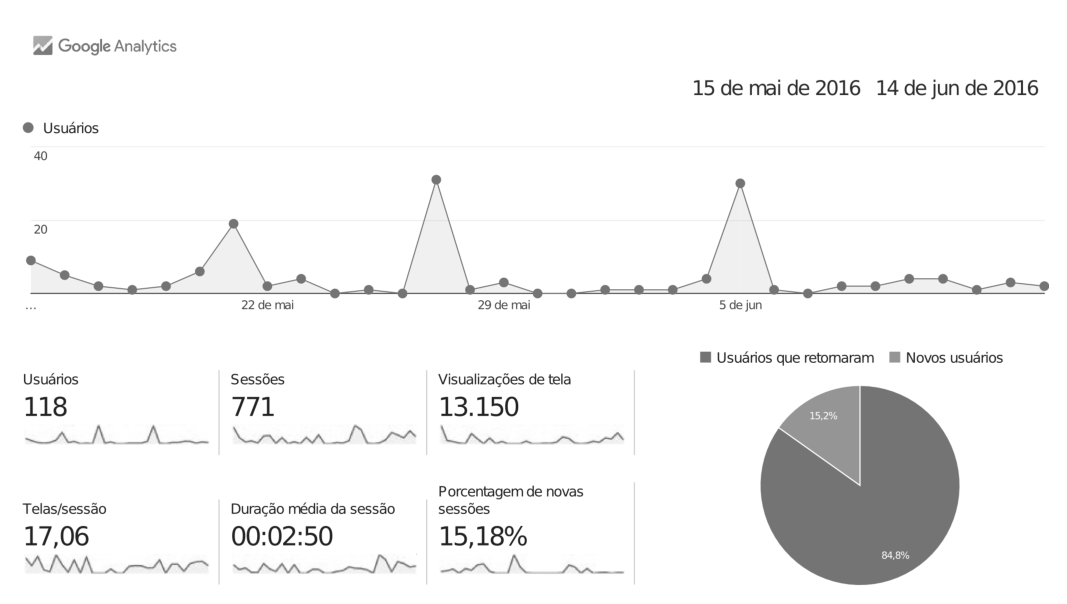
\includegraphics[width=0.8\textwidth]{figuras/analytics_acesso.eps} 
  \caption{Gráficos gerados pelo Google \textit{Analytics}.}
  \label{google_analytics}
\end{figure}

A partir do Google \textit{Analytics} foi possível classificar o principal público do aplicativo através de informações como o sexo, idade e monitoramento do aplicativo como de suas exceções (\textit{crash}) e quais são as telas visualizadas pelos usuários. Como pode ser observado na figura com a utilização do sistema Google \textit{Analytics} foi possível verificar a quantidade usuários do sistema, o tempo de duração média das sessões dos usuários, o percentual de novas sessões dentre outras informações pertinentes sobre a utilização do sistema.

\section*{Considerações finais sobre o capítulo}

\noindent Neste capítulo foi apresentado os resultados obtidos pela implantação do sistema ``\acrshort{uft} Serviços'', sendo apresentado o acordo de nível de serviço (SLA), o \textit{software}, os resultados dos testes realizados e as ferramentas de monitoramento.

Os resultados apresentados neste capítulo foram bastante satisfatórios pois foi possível ter uma visão geral sobre o potencial que aplicação terá a longo prazo. A implantação final do sistema ``\acrshort{uft} Serviços'' em produção irá proporcionar um sistema com desempenho satisfatório, uma boa taxa de aceitação devido ao excelente resultado obtido obtido pela aplicação do SUS e um ambiente de teste e monitoramento para a verificação do comportamento da aplicação durante a utilização dos usuários.
